% 中文正文（逐段忠实翻译自英文版 section01；公式照抄未改）

自 20 世纪 60 年代末斯坦福直线加速器中心的深度非弹性散射实验以来，质子的结构已在
各种硬散射过程中得到探测~\cite{Gao:2013xoa}。其结果是夸克与胶子（部分子）的动量分布
和关联，以及分布振幅等。部分子物理本质上涉及光锥关联：所有夸克与胶子场沿光锥分开，
而光锥由真实的闵可夫斯基时间 $t$ 定义。这些信息对于理解质子的非微扰结构极为有用，
例如可用于计算大型强子对撞机上希格斯产生的截面~\cite{science}。

从基本理论量子色动力学（QCD）出发计算部分子物理一直很困难。原则上，光锥关联最好用
光前坐标下质子的波函数来计算~\cite{brodsky}。然而，尽管多年努力，现实的光前质子波函数
至今尚未建立。另一方面，在欧氏格点上表述的非微扰 QCD 中，无法直接计算依赖时间的
关联，只能计算部分子分布和分布振幅的矩——它们是局域算符的矩阵元素。然而由于技术上的
原因，更高阶矩的困难显著增大~\cite{negele}。

本文给出一种通过洛伦兹助推在欧氏格点上直接计算部分子物理的方法。为演示这一点，
考虑质子中的夸克分布，
\begin{eqnarray}
   q(x, \mu^2) &=& \int \frac{d\xi^-}{4\pi} e^{-ix\xi^-P^+}  \langle P|\overline{\psi}(\xi^-)
   \gamma^+ \\
   && \times \exp\left(-ig\int^{\xi^-}_0 d\eta^- A^+(\eta^-) \right)\psi(0) |P\rangle \nonumber \ ,
\end{eqnarray}
其中核子动量 $P^\mu$ 沿 $z$ 方向，$P^\mu = (P^0, 0, 0, P^z)$；$\xi^\pm
=(t \pm z)/\sqrt{2}$ 是以真实时间 $t$ 定义的轻锥坐标；$\mu^2$ 是重正化标度；
$A^+$ 是基础表示下的胶子势矩阵；$\psi$ 是味道为 $q$ 的夸克场。上式沿 $z$ 方向
是助推不变的，即与 $P^z$ 无关；特别地，它在静止系（$P^z=0$）中成立。

为找到在欧氏格点上计算 $q(x,\mu^2)$ 的途径，有必要展示光锥关联的起源：部分子分布
也可用局域扭度2算符表述，其定义为
\begin{equation}
     O^{\mu_1...\mu_n}= {\overline \psi}\gamma^{(\mu_1}iD^{\mu_2} ... iD^{\mu_n)} \psi
                 - {\rm trace} \ ,
\end{equation}
其中 $(\mu_1...\mu_2)$ 表示所有指标对称化；迹项包含至少带一个度规张量因子
$g^{\mu_i \mu_j}$ 的算符乘以维数为 $(n+2)$、具有 $n-2$ 个洛伦兹指标的算符，等等。
它在质子态中的矩阵元素为
\begin{equation}
    \langle P|O^{\mu_1...\mu_n}(\mu^2)|P\rangle =
    2a_n(\mu^2) (P^{\mu_1} ... P^{\mu_n} - {\rm trace}) \ ,
\end{equation}
且当 $n$ 为偶数时，部分子分布通过 $\int dx x^{n-1} q(x, \mu^2)
= a_n(\mu^2)$ 与局域矩阵元素相联系。取式~(3) 中所有分量均为 $+$ 分量，即可恢复
式~(1) 中部分子分布的时间依赖关联：
\begin{equation}
   \langle P|O^{+...+}(\mu^2)|P\rangle =2 a_n(\mu^2) P^+...P^+ \ .
\end{equation}
因此，光锥关联在\textit{运动学上}与核子四动量的 $+$ 分量相连。

为消除时间依赖，我们考虑 $\mu_1=\mu_2=...=\mu_n=z$ 的扭度2算符在大 $P^z$
核子态中的矩阵元素。此时
\begin{equation}
   O^{z...z} = {\overline \psi}\gamma^{z}iD^{z} ... iD^{z} \psi - {\rm trace} \ ,
\end{equation}
其中迹项同样只含至多带 $n-2$ 个 $z$ 的算符。根据洛伦兹对称性，迹项的矩阵元素至多是
$(P^z)^{n-2}$ 乘以 $\Lambda^2_{\rm QCD}$。类似地，式~(3) 右边为
$2a_n(\mu^2)\left[(P^z)^n-\lambda M^2(P^z)^{n-2}-...\right]$，其中 $\lambda$ 是数量级
为 1 的数，$M$ 是核子质量，……表示 $P^z$ 幂次更低的项。于是我们得出结论：
\begin{eqnarray}
     && \langle P| {\overline \psi}\gamma^{z}iD^{z} ... iD^{z} \psi|P\rangle
       = 2a_n(\mu^2) (P^z)^n\times \left[ 1 \right.\\ && \left.+ {\cal O}\left(\Lambda^2_{\rm QCD}/(P^z)^2,  M^2/(P^z)^2\right)\right] \nonumber
\end{eqnarray}
即除首项外，其余各项在大 $P^z$ 极限下均为幂次压低。

把上述结果反解为一个不依赖时间的非定域表达式，在大 $P^z$ 极限下我们得到
\begin{eqnarray}
   q(x,\mu^2, P^z) &=& \int \frac{dz}{4\pi} e^{izk^z}  \langle P|\overline{\psi}(z)
   \gamma^z \\
   && \times \exp\left(-ig\int^{z}_0 dz' A^z(z') \right)\psi(0) |P\rangle \nonumber
 \\ && + {\cal O}\left(\Lambda^2/(P^z)^2,  M^2/(P^z)^2\right) \ ,  \nonumber
\end{eqnarray}
其中 $x= k^z/P^z$。
理解上述结果的一个直观方式，是考察连接 $(0,0,0,z)$ 与坐标原点的线段的洛伦兹变换。
当助推速度趋于光速时，类空线段向光锥方向倾斜。当然，它不可能真正落在光锥上，因为
不变长度不会因任何助推而改变。然而，这种轻微的偏离光锥只引入渐近消失的幂次修正。

直观地说，式~(1) 的部分子分布可视为核子处于静止系、而探针以光速运动的情形，因而有
光锥关联；另一方面，式~(7) 的分布则来自以光速运动的核子上的静止探针。后一情形对应于
虚光子动量只含空间分量 $q^\mu = (0, Q)$、核子动量为 $P^z \sim Q/2x$ 的参考系中的深度
非弹性散射。把 $\gamma^z$ 换成 $\gamma^z\gamma_5$，还可以得到夸克螺旋度分布的类似
表达式。至于胶子分布，我们有
\begin{eqnarray}
g(x,\mu^2, P_z) = \int \frac{dz}{4\pi k^z}
e^{izk^z} \langle P|F^{3\mu}(z)  \\
\times \exp\left(-ig \int^z_0 dz' A^z(z')\right)
F^{~3}_\mu(0)|P\rangle \nonumber
\end{eqnarray}
在大 $P^z$ 极限下成立，其中 $A^z$ 是伴随表示下的矩阵，$i$ 对横向方向求和。
类似地，我们有极化胶子分布
\begin{eqnarray}
\Delta g(x,\mu^2, P_z) = i\int \frac{dz}{4\pi k^z}
e^{izk^z} \langle P|F^{3\mu}(z)  \\
\times \exp\left(-ig \int^z_0 dz' A^z(z')\right)
\tilde F^{~3}_\mu(0)|P\rangle \nonumber \ ,
\end{eqnarray}
由此积分可得 $\Delta G$（$\tilde F^{\mu\nu} = 1/2 \epsilon^{\mu\nu\alpha\beta}F_{\alpha\beta}$）。不过，我们还发现了另一种无需显式完成该积分即可在格点上
计算 $\Delta G$ 的方法~\cite{Ji:2013fga}。

\begin{figure}[hbt]
\begin{center}
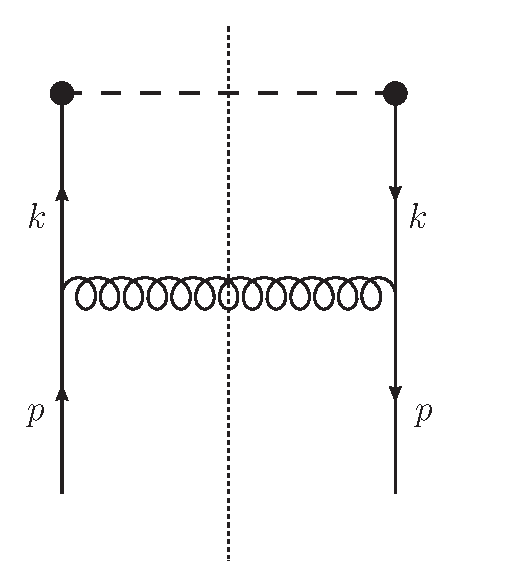
\includegraphics[width=30mm]{images/pdf.eps}
\caption{$A^z=0$ 规范下式~(7) 部分子分布的单圈修正。}
\label{phqcorrection}
\end{center}
\end{figure}

在场论中取无穷大动量极限是一个微妙的过程：必须以正确的极限程序妥善处理圈积分中的
紫外（UV）发散。在我们的情形中，需要在重正化程序之后取极限，而式~(1) 的标准光锥
结果则是先取 $P^z\rightarrow \infty$ 再作重正化。因此用现代语言来说，光锥分布是式~(7)
那个量的有效场论：其间微扰论中出现大对数 $\ln P^z$，可通过匹配条件把它转化为光锥分布
中标准的重正化标度依赖~\cite{jizhangzhao}。在物理的 $A^z=0$ 规范下计算单圈修正即可看出
两种极限的相互影响（见图~1）：
\begin{eqnarray}
    q(x, \mu^2, P^z) = \frac{\alpha_s}{2\pi}T(x) ~\frac{\Lambda}{P^z}+    \frac{\alpha_s}{2\pi} P(x) ~ \ln\frac{\Lambda P^z}{\lambda^2}
\end{eqnarray}
其中 $\Lambda = \sqrt{\mu^2 + (1-x)^2(P^{z})^2}-(1-x)P^z$，$\lambda$ 是红外质量截断，
$\mu^2$ 是紫外截断（重正化标度）；$T(x) =C_F x/(1-x)^2$，而 $P(x) = C_F (1+x^2)/(1-x)$
（$C_F=4/3$）正是标准的 Altarelli-Parisi 演化核~\cite{AP}。若先取
$P^z\rightarrow \infty$，则 $\Lambda \sim \mu^2/P^z$，第一项被幂次压低，第二项即为标准
AP 结果。然而若先取 $\mu^2\rightarrow \infty$（这正是我们所关心的），第一项线性发散，
第二项则变为 $\ln (\mu P^z/\lambda^2)$。两种极限的联系体现为下面这个在计及幂次修正之前的
因子化定理：
\begin{equation}
    q(x, \mu^2, P^z)  = \int^1_x \frac{dy}{y} Z\left(\frac{x}{y},\frac{\mu}{P^z}\right) q(y, \mu^2)
\end{equation}
其中 $Z$ 具有按 $\alpha_s$ 的微扰展开
\begin{equation}
             Z(x, \mu/P^z) = \delta (x-1) + \frac{\alpha_s}{2\pi} Z^{(1)}(x, \mu/P^z) + ...
\end{equation}
且 $Z^{(1)} = T(x)(\mu/P^z) + P(x)\ln (P^z/\mu)$。先取 $P^z \rightarrow \infty$ 给出
$Z(x, \mu/P^z) = \delta(x-1)$。这样，$q(x,\mu^2,P^z)$ 中对 $P^z$ 的大对数依赖便可借助上述
匹配条件转化为重正化标度依赖。
在格点上，匹配必须用标准方法重新计算到常数精度~\cite{ren}。

因此，可以在格点上利用式~(11) 计算部分子分布 $q(x,\mu^2)$：只需在不断增大的 $P^z$
态中测量不依赖时间的非定域夸克关联函数 $\overline{\psi}(z)\gamma^zL(z,0)\psi(0)$，其中
$L(z,z_0) = \exp\left(-ig\int^{z}_{z_0} dz' A^z(z') \right)$（最大值约 $\sim 1/a$，$a$
为格距）。
格点上最小与最大的动量分别为 $1/L_z a$ 和 $1/a$，故能分辨的最小 $x$ 为 $1/L_z$，这里
$L_z$ 是 $z$ 方向的格点数。要达到 $x = 10^{-2}$，需要约 $100$ 个格点。另一方面，本方法
能够对大 $x$ 区的部分子给出合理描述，这部分信息由分布的高阶矩所强调。因此在某种意义上，
该方法与传统矩方法是互补的。另外，固定 $x$ 时大 $P^z$ 意味着大 $k^z$，从而 $z$ 很小。
于是，快速运动的核子在 $z$ 方向经历洛伦兹收缩，要研究其纵向结构就需要越来越高的分辨率
（如谱学计算中所用的各向异性点阵~\cite{Edwards:2011jj}）。

上述方法可以推广到强子物理中任何光锥关联。一份有趣物理量的不完全清单包括：
\begin{itemize}
\item{广义部分子分布（GPD）~\cite{Ji:1996ek}：使用同样的扭度2算符，但外态是非对角的。
例如，GPD $E(x,\xi, t)$ 和 $H(x, \xi, t)$ 可由如下矩阵元素计算：
\begin{eqnarray}
  F(x, \xi, t, P^z) &=& \int \frac{dz}{2\pi} e^{-izk^z}\langle P'|\overline\psi(-z/2)\gamma^z \\ && \times L(-z/2,z/2)\psi(z/2)|P\rangle \nonumber
\end{eqnarray}
其中 $\vec{P}'+\vec{P}=2(0,0,\overline{P}^z)$，并在 $P^z\rightarrow \infty$、
$\xi= (P^{z'}-P^z)/\overline{P}^z$、$x=k^z/\overline{P}^z$ 固定的极限下。类似地，通过插入不同的狄拉克矩阵并选取不同的核子极化态，可以得到其他扭度2 GPD。
于是，人们现在无需模型假设便能细致探索对 $x$、$\xi$ 和 $t$ 的三维依赖~\cite{Hagler:2003jd}。}

\item{横动量依赖（TMD）部分子分布~\cite{collins}。例如对狄拉克矩阵 $\gamma^z$，我们可以
得到如下 TMD：
\begin{eqnarray}
  && q(x,k_\perp, P_z, \mu^2)\nonumber \\ &=& \int \frac{dz}{4\pi} d^2\vec{r}_\perp e^{i(zk^z+\vec{k}_\perp \vec{r}_\perp)}  \langle P|\overline{\psi}(\vec{r}_\perp,z)
    \\ && \times L^\dagger\left(\pm\infty; (\vec{r}_\perp,z)\right)\gamma^z L(\pm\infty; 0)\psi(0) |P\rangle \nonumber
\end{eqnarray}
其中 $P^z$ 必须很大，且 $L\left(\pm\infty; (\vec{r}_\perp, z)\right) = e^{-ig\int^{\pm\infty}_{z} dz' A^z(\vec{r}_\perp, z')}$。此时对 $P^z$
的依赖含有大对数 $\ln P^z$，在大 $P^z$ 极限下并不消失，因此显式地写在函数中。
可以为 $P^z$ 导出演化方程~\cite{collins}。
这里的规范链只沿 $z$ 方向从夸克场所在位置延伸到 $\pm \infty$，因而只涉及规范势的
$A^z$ 分量。$\pm\infty$ 对应探测分布的两种不同运动学条件。在规范势在无穷远处为零的规范
选择下，上式是规范不变的。但对有限格点并对所有规范取平均时，两条规范链必须由另一条沿横向空间方向的规范链
$L((\vec{r}_\perp, \pm\infty);(0,\pm \infty))$ 连接起来。用其他狄拉克结构定义的 TMD 有类似的
表达式。已有探索性工作在格点上研究了 TMD 分布的 $x$ 阶矩，其中规范链取为空间方向的
U 形（staple）路径~\cite{Musch:2010ka}。与光锥运动学的联系通过不变分解而非助推实现，
尽管这些分布本身定义在大 $P^z$ 处。}

\item{维格纳（Wigner）分布~\cite{viewing}，它是 GPD 与 TMD 两者的生成函数。其定义来自夹在非前向核子态之间的
TMD 算符。于是可以在大的 $P^z$ 极限下计算它们，例如
\begin{eqnarray}
  &&  W(x,k_\perp,b_\perp, P^z, \mu^2) \\ &&
  = \int \frac{dz}{4\pi} d^2\Delta_\perp d^2\vec{r}_\perp e^{-i\Delta_\perp \cdot b_\perp} e^{i(zk^z+\vec{k}_\perp \vec{r}_\perp)}\nonumber
    \\ && \times \langle P'|\overline{\psi}(\vec{r}_\perp,z)L^\dagger(\pm\infty; (\vec{r}_\perp,z))\gamma^z L(\pm\infty; 0)\psi(0) |P\rangle \nonumber
\end{eqnarray}
其中 $\Delta_\perp =(P'-P)_\perp$；同样，为保证有限格点上的规范不变性还需要一条横向
规范链。我们还注意到，在大的 $P^z$ 极限下，$P^z$ 依赖并不消失。}

\item{光锥振幅，即强子态与 QCD 真空之间、夸克与胶子插值场光锥关联的矩阵元素。我们现在可以把它们作为大动量极限下空间关联的矩阵元来计算。例如，$\pi^+$
介子的领头光锥振幅即为下式的大 $P^z$ 极限：
\begin{equation}
\phi_0(x, P^z) 2P^z = \int \frac{dz}{2\pi} e^{izk^z}
\langle 0|\overline{d}(0)\gamma^z\gamma_5
L(0,z)u(z)| \pi^+(P)\rangle \ .
\end{equation}
这些光锥振幅可以通过诸如形状因子等硬遍举过程加以探测~\cite{Lepage:1980fj,Belitsky:2002kj}。
文献中对 $\phi_0(x)$ 振幅的 $x$ 依赖已有诸多讨论。}

\item{光锥波函数。在光前坐标下，核子态可以写成带有波函数振幅的无穷多福克态之和~\cite{brodsky}。
在一系列文章~\cite{Ji:2002xn}中，我们系统分类了直到四部分子的 $\pi$ 介子与质子波函数振幅，
并把它们同光锥及横向方向上夸克胶子关联的矩阵元素联系起来。当沿光锥方向从场所在位置向无穷远
插入光锥规范链时，所有这些振幅都是规范不变的。这些振幅同样可在格点上计算：取类似关联函数
的无穷动量极限，其中场由沿 $z$ 方向延伸到无穷远的规范链连接。一个重要应用是 B 介子的遍举衰变——许多因子化公式都以光锥波函数作为衰变振幅的一部分而被导出~\cite{li}。}

\item{高扭度部分子分布。非极化、纵向极化与横向极化核子的扭度2、3、4部分子分布完整清单
已在文献中给出~\cite{Ellis:1982cd}。它们的夸克胶子场都沿光锥分开。按照本文的精神，它们都可以由 $P^z \rightarrow \infty$ 极限下沿 $z$ 方向带有规范链的相关空间关联函数得到。特别是，
喷注淬灭参数 $\hat q$ 或许可以用这种方式计算~\cite{Majumder:2012sh}。}

\item{……}

\end{itemize}
看到这些量如今可以在格点 QCD 计算中得到探索，将是十分令人期待的。

总之，我已证明：夸克与胶子的光锥关联可以通过把空间关联的矩阵元素助推到大动量来计算。
这对于这些实验可观测量——过去从第一性原理处理非常困难——的格点 QCD 计算尤为有用。
诚然，在格点上研究大动量的强子在计算上仍具挑战性，但随着计算能力的持续提升，这至少是
可以实现的目标。
